\documentclass[letterpaper,10pt,conference]{ieeeconf}
\IEEEoverridecommandlockouts
\overrideIEEEmargins
\usepackage{graphicx}
\usepackage{amsmath,amssymb}
\usepackage{booktabs}
\usepackage{multirow}
\usepackage{xcolor}
\usepackage{url}
\usepackage{dblfloatfix}
\usepackage{float}
\newcommand{\jointseq}{Joint-Space Sequence}
\newcommand{\cartseq}{Cartesian-Space Sequence}
\newcommand{\method}{Motion Program}
\newcommand{\methodfull}{Symbolic Motion Program}
\newcommand{\traj}{Trajectory Sketching}
\newcommand{\trajfull}{Geometric Trajectory Sketching}
\newcommand{\TODO}[1]{\textcolor{red}{[TODO: #1]}}

% --- float placement: at most one full-width and one column float per page
\setcounter{topnumber}{1}
\setcounter{bottomnumber}{1}
\setcounter{totalnumber}{1}
\setcounter{dbltopnumber}{1}
\renewcommand{\topfraction}{0.70}
\renewcommand{\bottomfraction}{0.35}
\renewcommand{\dbltopfraction}{0.70}
\renewcommand{\textfraction}{0.22}
\renewcommand{\floatpagefraction}{0.80}
\renewcommand{\dblfloatpagefraction}{0.80}

\title{Language-Executable Motion Abstractions for Recognizable Robot Gestures}
\author{Anonymous Authors\thanks{Anonymous submission. Identifying links are omitted for double-anonymous review.}}

\begin{document}
\maketitle
\thispagestyle{empty}
\pagestyle{empty}

\begin{abstract}
Large language models can describe familiar gestures, but turning this knowledge into executable robot motion requires embodiment-specific spatial and temporal understanding. We propose two language-executable motion abstractions: the \textit{\methodfull{}}, which composes named \texttt{pose}, \texttt{movement}, and \texttt{path} components, and the \textit{\trajfull{}}, which emits $xyzrpy$ waypoints only for the links a cue requires. To evaluate them we assemble 30 communicative cues spanning head, deictic, emblematic, and depictive families, and author reference motions for cues on five embodiments---Humanoid, Tiago, Single Arm, Stretch, and Roomba---establishing that each cue is expressible (92.7\%) on each body. In a cue-identification study with \TODO{N} observers, both abstractions exceed the dense \cartseq{} and \jointseq{} baselines on all five embodiments: \traj{} reaches 66.0\% and \method{} 57.3\%, against 45.3\% and 34.7\%. Neither matches the human-authored references, and the residual failures differ by morphology. On human-like bodies, recognition falls when small orientation details such as palm facing are wrong, even when the intended pose and path are otherwise correct (\textit{misspecification}). On bodies without human form and with a small action space, such as Stretch and Roomba, the generated motions are not incorrect but lack the expressive richness required to distinguish one cue from another (e.g., \texttt{raise\_fists\_victory} vs.\ \texttt{hands\_up\_surrender}; \textit{underspecification}).
\end{abstract}

\section{Introduction}
Robot motion serves not only to perform functional tasks, such as lifting a cup, but also to communicate internal states, including intent, perception, knowledge, and emotion. We use \emph{gesture} to denote a culturally conventionalized subset of such communicative motion: movements whose nuanced meanings are broadly shared within a cultural community. The primary measure of a gesture is its \emph{recognizability}---whether an observer recovers its intended meaning~\cite{dragan2013legibility}. Recognizability depends jointly on body pose, movement direction, speed, repetition, and other spatial and temporal factors. Gesture generation is therefore a constrained motion-synthesis problem, not merely the production of feasible movement.

\begin{figure}[!t]
\centering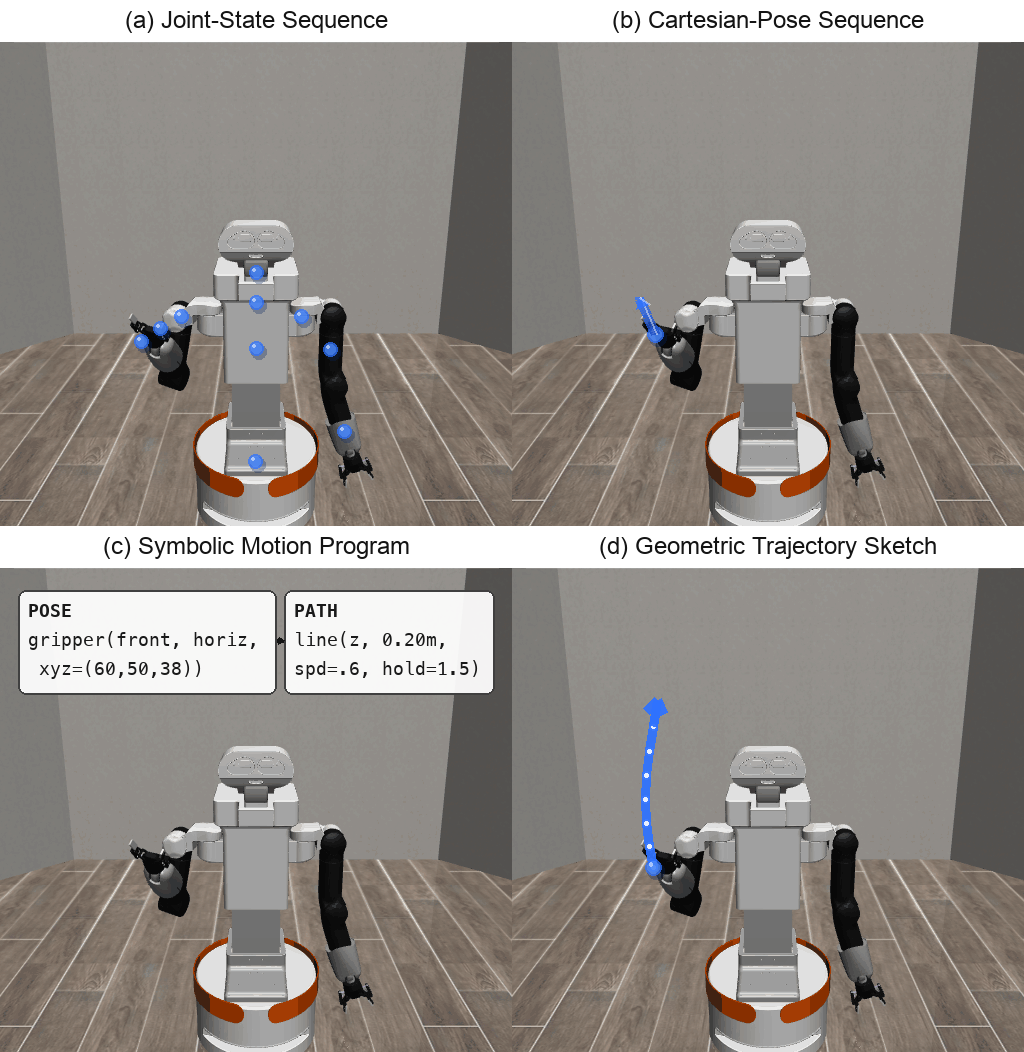
\includegraphics[width=.98\columnwidth]{figures/figure2_interfaces.png}
\caption{The four interfaces trade robot-specific detail for abstraction and selective focus. The \jointseq{} serializes calibrated joint states; the \cartseq{} serializes link/EE poses and uses IK; the \method{} emits factorized \texttt{pose} and \texttt{path} symbols; and the \traj{} emits sparse EE/base-path handles retargeted by a controller. The latter two defer morphology grounding while preserving symbolic pose semantics or path geometry, respectively.}
\label{fig:interfaces}
\end{figure}

\begin{figure*}[!t]
\centering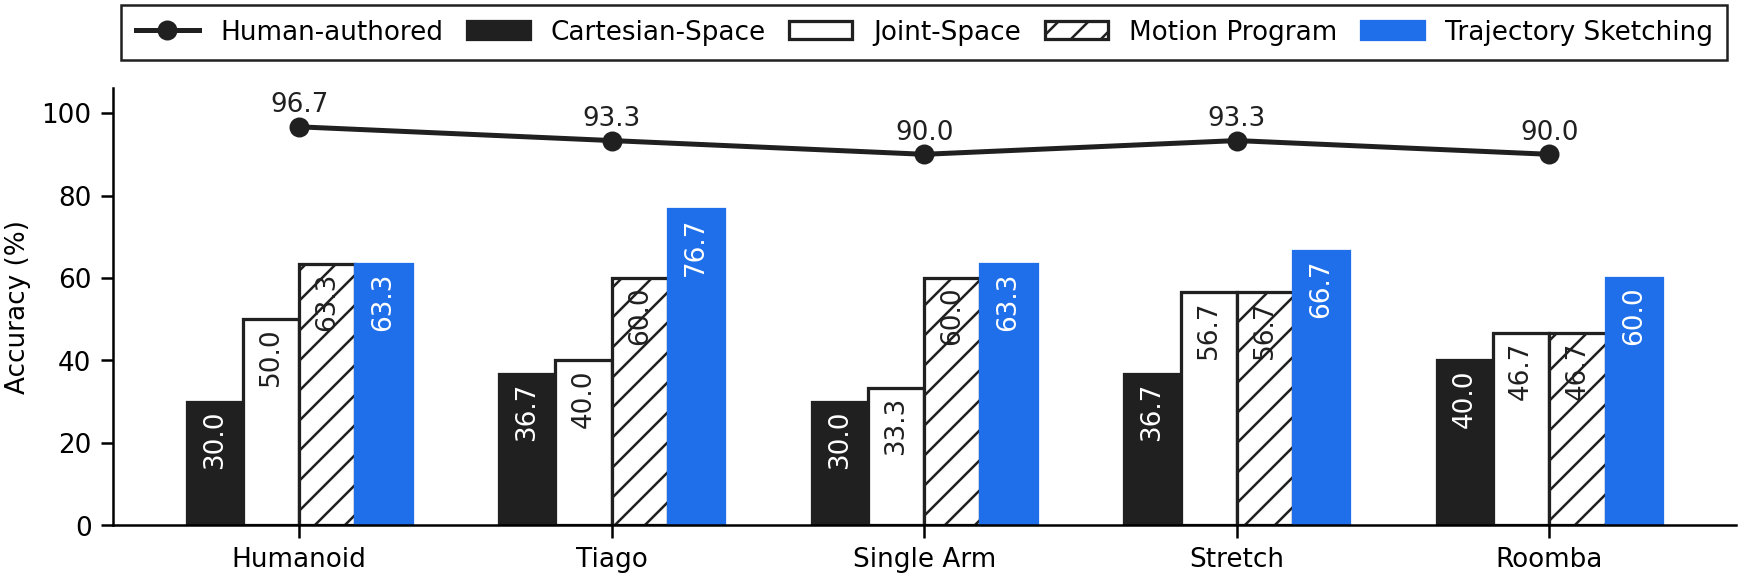
\includegraphics[width=.96\textwidth]{figures/figure1_human_eval.png}
\caption{Main result: human cue-identification accuracy. Numbers above the black line give human-authored accuracy. Generated interfaces are bars. \traj{} is strongest overall, but the profile varies substantially by embodiment.}
\label{fig:human}
\end{figure*}

Existing pipelines have largely treated a human author or human demonstration as a prerequisite for producing recognizable gestures. Communicative motions are therefore authored cue by cue~\cite{kopp2006bml,salem2012gesture,chidambaram2012gesture} or learned from human motion~\cite{kucherenko2020gesticulator,yoon2020trimodal,liu2022beat}. The former preserves semantic control but repeats design work for every cue and body. The latter scales examples, but its human skeleton and motion statistics do not specify how a single arm or mobile base should communicate the same meaning. LLM-based robot systems can reuse broad language knowledge, yet they often compose an API whose skills, arguments, and controllers were designed in advance~\cite{brohan2023rt2,liang2023cap,huang2023voxposer}. These pipelines leave an abstraction question unresolved: \emph{what should the model generate, and what should it defer to embodiment-specific execution, so that gesture knowledge remains recognizable?}

We evaluate the abstraction question with 30 diverse cues and five bodies, which we refer to throughout by the short names used in all figures and tables: Humanoid (Unitree G1), Tiago (PAL Robotics), Single Arm (KUKA IIWA), Stretch (Hello Robot), and Roomba (iRobot). The set ranges from simple head and arm movements (e.g., \texttt{point\_you}), through cues that require precise body-relative placement or orientation (e.g., \texttt{air\_quotes}), to depictive motions that trace an object or shape (e.g., \texttt{depict\_flying\_bird}). Human-authored realizations provide a constructive reference that these meanings can be expressed across the five bodies. As Fig.~\ref{fig:interfaces} shows, we compare two numerical baselines with two abstraction strategies. The \jointseq{} and \cartseq{} baselines serialize full joint-space or task-space state. The \method{} instead composes body-relative \texttt{pose}, geometric \texttt{path}, and movement-dynamic factors as editable symbols. The \traj{} uses Cartesian-style $xyzrpy$ values, but serializes only the links that must move. The abstractions therefore test two ways to reduce the generation problem: semantic factorization and selective geometric focus.

Human-authored motions reach 92.7\% recognition across bodies, including non-anthropomorphic realizations such as \texttt{depict\_flying\_bird} with a Roomba embodiment. Even the most recognizable LLM interface, \traj{}, achieves only 66.0\% mean recognition, 26.7 percentage points below the human-authored reference. This deficit occurs on all five embodiments, ranging from 16.6 points on Tiago to 33.4 points on Humanoid. The abstraction-based interfaces nevertheless outperform the strongest numerical baseline on every embodiment; the largest gains occur on Tiago (36.7 points) and Single Arm (30.0 points). \traj{} obtains the highest, or ties for the highest, generated-motion recognition on all five bodies, but still omits or misspecifies cue-bearing details such as palm and EE orientation and, on Roomba, uses fewer coordinate directions than human-authored motion (32\% versus 38\%). \method{} provides a complementary efficiency advantage: it reduces mean output from 1,890.2--1,961.8 tokens for dense sequences to 73.2 tokens and names factors that a person can inspect and correct. Our contributions are:
\begin{itemize}
\item \textbf{Human-authored cross-embodiment references} -- 30 cues on five bodies, recognized 92.7\% of the time, including on non-anthropomorphic ones.
\item \textbf{Two language-executable abstractions} -- symbolic factors and selective geometry, both more recognizable than the dense numeric baselines on all five bodies.
\item \textbf{Misspecification and underspecification} -- we define two failure modes and use them to distinguish the dominant failure pattern on human-like bodies from the one on bodies without human form.
\end{itemize}

\section{Related Work}
\textbf{Communicative Robot Behavior and Gesture.} Communicative motion makes intent, attention, affect, or reference observable to another agent~\cite{dragan2013legibility}. Prior systems encode such behavior through authored multimodal specifications and robot-specific cues~\cite{kopp2006bml,salem2012gesture,chidambaram2012gesture}, or learn gesture statistics from paired human speech and motion~\cite{kucherenko2020gesticulator,yoon2020trimodal,liu2022beat}. Authoring preserves semantic judgment but scales poorly across cues and bodies. Human-motion distillation scales generation, but usually assumes a human-like skeleton and emphasizes naturalness or speech synchrony. Our setting instead holds communicative intent fixed while varying morphology from a humanoid to a planar mobile base, making embodiment-specific realization the object of study.

\textbf{Language-Executable Motion Abstractions.} Motion primitives compress control into reusable parameters: DMPs~\cite{ijspeert2013dmp}, probabilistic primitives~\cite{paraschos2013promp}, and task-parameterized models~\cite{calinon2016tpgmm} each preserve different trajectory structure. Language-conditioned systems map instructions to demonstrations~\cite{stepputtis2020lcil}, policies~\cite{brohan2023rt2}, code~\cite{liang2023cap}, spatial objectives~\cite{huang2023voxposer}, DMP parameters~\cite{dai2026lmp}, or contact costs~\cite{ling2026impact}. Language feedback can also correct assistive motions~\cite{broad2017corrections}, plans~\cite{sharma2022correcting}, and policies~\cite{shi2024yell}; these methods nevertheless assume a controller, skill library, task space, or correction vocabulary. We treat the executable interface itself as the experimental variable and ask which abstraction preserves cue-bearing pose and movement across embodiments.

\section{Task Definition}
\subsection{Cue Set}
We select 30 cues to cover both semantic breadth and physical diversity. The set spans head/face, deictic, emblematic, and depictive gestures (Table~\ref{tab:categories}) and deliberately varies the carrier needed for recognition: head rotation, body-relative arm placement, EE or palm facing, bilateral coordination, repetition, and multi-stage paths. This coverage is necessary because the five embodiments expose different subsets of those channels; a benchmark solvable by one hand pose or one path shape would not test cross-body generation. Human-authored feasible motions confirm that every cue can be expressed on every body, while the complete cue inventory appears in Supplementary Table~\ref{tab:all-cues}. The cue set therefore tests whether each interface can express the same intended meaning using the motion capabilities available on each robot.

\begin{table*}[!t]
\caption{Generated-method cue-identification accuracy by cue family and embodiment (\%). Values pool \jointseq{}, \cartseq{}, \method{}, and \traj{}; human-authored references are excluded.}
\label{tab:categories}
\centering\small
\begin{tabular}{llccccc}\toprule
Examples & Cue family & Humanoid & Tiago & Single Arm & Stretch & Roomba\\\midrule
\texttt{nod\_yes}, \texttt{cover\_yawn\_sleepy} & Head and face & \textbf{82.1} &67.9&64.3&64.3&53.6\\
\texttt{point\_you}, \texttt{beckon\_come\_here} & Deictic / directed &39.3&53.6&32.1&46.4&\textbf{60.7}\\
\texttt{shrug\_idk}, \texttt{arms\_open\_welcome} & Emblematic pose &32.5&47.5&\textbf{52.5}&47.5&40.0\\
\texttt{depict\_lion}, \texttt{depict\_flying\_bird} & Depictive / iconic &\textbf{62.5}&45.8&33.3&\textbf{62.5}&41.7\\\bottomrule
\end{tabular}
\end{table*}

\begin{figure*}[!b]
\centering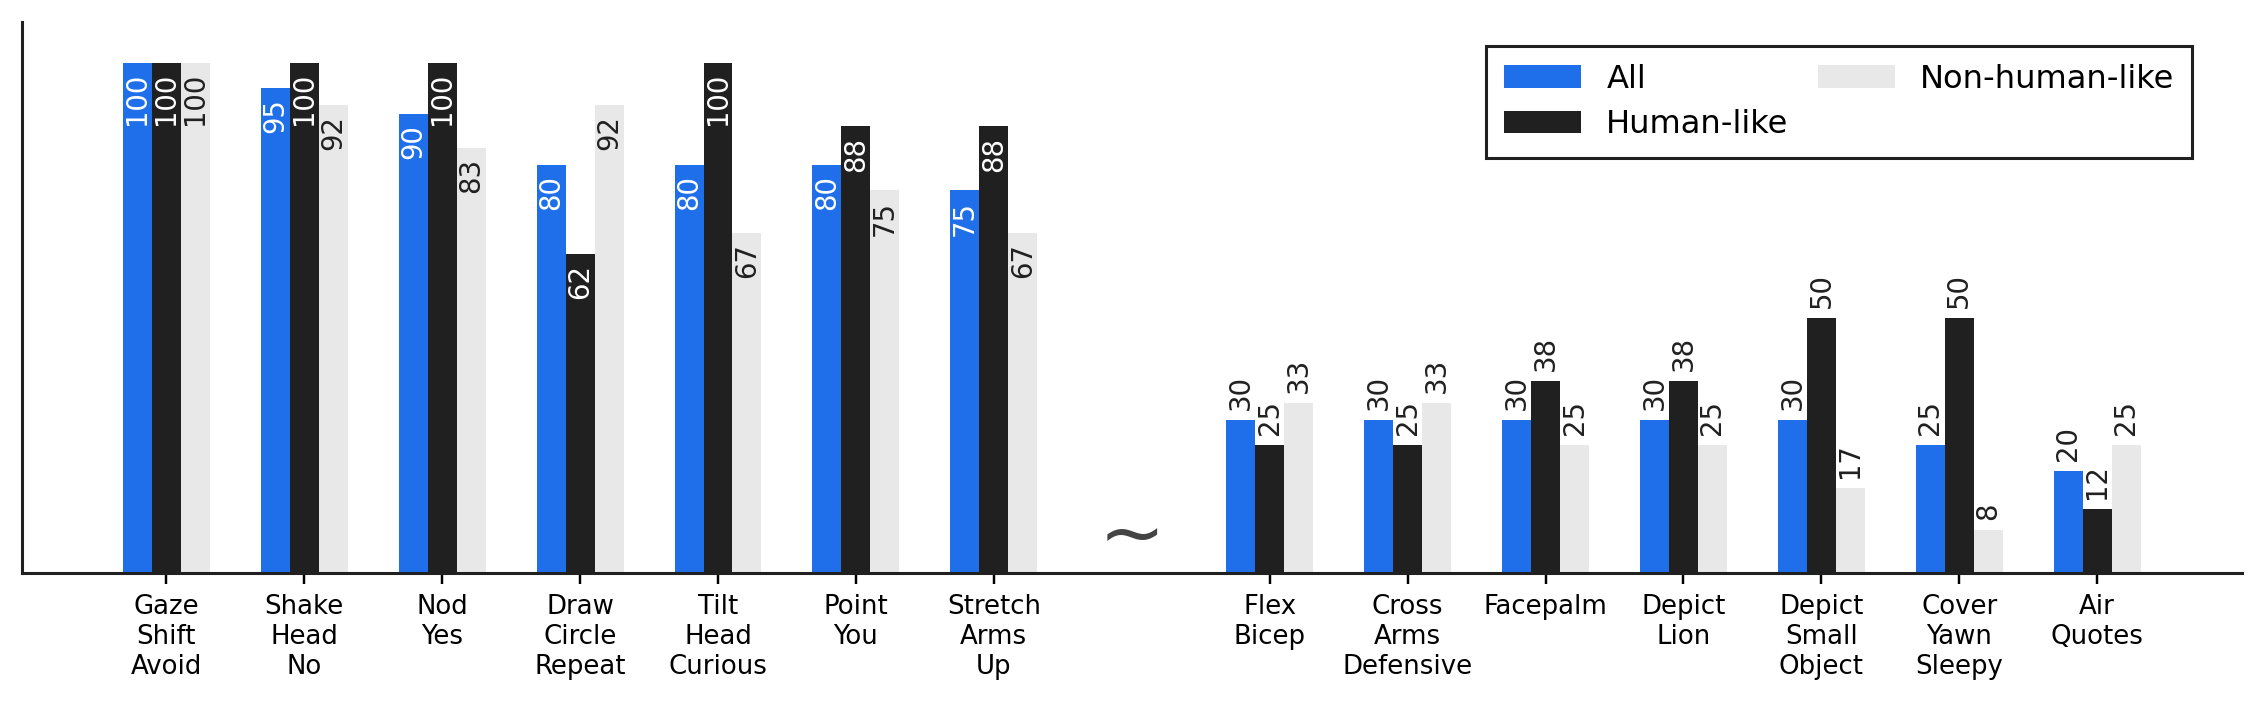
\includegraphics[width=.96\textwidth]{figures/figure16_cue_difficulty.png}
\caption{Recognition varies substantially by cue and embodiment type. The highest- and lowest-recognition cues are ranked by mean generated-method accuracy for human-like and non-human-like bodies.}
\label{fig:cue-difficulty}
\end{figure*}

\subsection{Abstraction Levels}
Among the many motion abstractions that can be expressed through language, we design two interfaces to test two directions of abstraction. \textbf{Numeric vs. Symbolic: the \methodfull{} (\method{})} replaces dense numerical states with named, composable motion attributes. \textbf{Whole vs. Targeted: the \trajfull{} (\traj{})} describes only the body parts that must move instead of serializing the full robot state. We compare these abstractions with two numerical baselines that output complete joint-space or Cartesian-space sequences~\cite{liang2023cap,huang2023voxposer}. Fig.~\ref{fig:interfaces} illustrates the four interfaces, and Supplementary Table~\ref{tab:grounding} summarizes their embodiment-specific implementations.

\subsubsection{\jointseq{}}
The \jointseq{} serializes calibrated robot joint states at every frame. It commits most directly to a particular embodiment and avoids an IK step, but it requires the model to coordinate all coupled joints and to preserve meaningful pose structure across the entire sequence.

\subsubsection{\cartseq{}}
The \cartseq{} serializes link or end-effector poses at every frame and delegates joint realization to inverse kinematics. It retains explicit geometric targets, but every answer is still a dense, embodiment-specific numerical sequence; a redundant robot can realize the same EE target through different joint branches.

\subsubsection{\methodfull{} (\method{})}
The \method{} is our first proposed abstraction and composes three components: \texttt{pose}, \texttt{movement}, and \texttt{path}. The \texttt{pose} component specifies a body or EE configuration; \texttt{movement} specifies how a body part or joint changes; and \texttt{path} specifies a Cartesian trace and its timing. Different motions, joint structures, and morphologies are represented by varying the attributes inside these components while retaining the same compositional format. Shared attributes include six directions---\texttt{front}, \texttt{back}, \texttt{left}, \texttt{right}, \texttt{up}, and \texttt{down}---and the Cartesian movement axes \texttt{x}, \texttt{y}, and \texttt{z}, which can be combined with extent, speed, repetition, and hold attributes to construct the requested motion.

\subsubsection{\trajfull{} (\traj{})}
The \traj{} is our second proposed abstraction and emits waypoints only for links that move away from the neutral configuration. Each waypoint is represented as an $xyzrpy$ target that an inverse-kinematics controller converts into joint angles. For redundant arms, the model can additionally specify an optional elbow-up or elbow-down configuration to select the intended IK branch. Links without emitted waypoints remain at their neutral states, so the model specifies the motion-relevant geometry without serializing the complete robot trajectory.

\subsection{Generation Setup}
All four interfaces are produced by a single model, Gemini~2.5~Pro, so that the output representation is the only variable. Decoding is fixed across interfaces at temperature $0.3$ with a 16{,}384-token output limit and the smallest thinking budget the model permits. Every interface receives the same cue name, the same embodiment description, and the same frozen set of human-authored few-shot exemplars for that body; only the output-format specification differs. We draw one generation per (cue, embodiment, interface) cell, giving $30\times5\times4=600$ generated motions, which are rendered alongside the 150 human-authored references. An output that fails to parse or to satisfy the format contract is resampled---three retries with exponential backoff per pass, with unresolved cells re-queued on the next pass---until every cell yields an executable motion, so no cell is dropped from the study. The two dense baselines request 16--32 frames at 8\,Hz with all parts or links sharing one frame count, so \jointseq{} and \cartseq{} are matched in temporal resolution. The five few-shot exemplars (\texttt{raising\_hand\_greeting}, \texttt{wave\_hi}, \texttt{bow\_greeting}, \texttt{blow\_kiss}, \texttt{circle\_temple\_crazy}) are disjoint from the 30 evaluated cues.

\subsection{Evaluation and Metrics}


One measure reports the \emph{outcome} and three report the \emph{cause}. Cue identification asks whether an observer recovers the intended meaning, and is the only measure of communicative success. It does not say what went wrong, so we add three diagnostics against the human-authored reference: the pose error localizes the failure to a body-relative position or a facing, and expression richness asks whether the motion recruits enough of the body to be told apart from other cues at all. The pose error is measured against a reference and is reported in Table~\ref{tab:factor-fidelity}; richness has no correct value and is reported against the human-authored level in Table~\ref{tab:diversity}.

\subsubsection{Human Cue Identification}
Each of the $30\times5\times5=750$ rendered motions---30 cues on five embodiments, for the four generated interfaces plus the human-authored reference---receives one binary judgment: shown the rendered motion together with its intended cue label, an observer reports whether the motion conveys that cue. \TODO{N} observers (\TODO{recruitment, demographics, compensation}) each judged \TODO{number} motions, with interface and provenance unlabeled and presentation order randomized. \TODO{state whether any cell was judged by more than one observer, and report agreement}. \TODO{IRB protocol}. Accuracies are reported with \TODO{95\% CIs} and interfaces compared with \TODO{test}.

Let $r_i\in\{0,1\}$ denote whether an observer recognizes rendered motion $i$ as its intended cue. Identification accuracy is
\begin{equation}
\mathrm{Acc}_{\mathrm{cue}}=\frac{1}{N}\sum_{i=1}^{N}r_i,
\end{equation}
where $N$ is the number of rated motions. This directly tests communicative success.

\subsubsection{Cue-Bearing Pose Error}
Recognition alone does not say \emph{which} part of a motion failed. We therefore compare every generated motion with the human-authored reference on the named factors that carry a cue, and we read each factor at the frame where it is visible: the \emph{peak pose}, the frame whose deviation from the neutral configuration is largest. Deviation is measured on both channels, because some carriers move only rotationally --- a nod leaves the head landmark in place while turning its frame:
\begin{equation}
D(t)=\max_{l\in L}\ \max\!\left(
\frac{\lVert \tilde{p}_{t,l}-\tilde{p}_{0,l}\rVert_2}{\tau_p},\
\frac{\angle\big(R_{t,l},R_{0,l}\big)}{\tau_r}\right),
\end{equation}
\begin{equation}
t^\star=\arg\max_t D(t),
\end{equation}
with $\tau_p=0.04$ in embodiment-normalized units and $\tau_r=5^\circ$, so the two channels enter in units of their own detection threshold. A trace with $D\equiv 0$ holds a single pose and any frame serves.

\textbf{Location} is reported per axis, in workspace percentile points, so that one point means the same thing on every body and for every cue. With $[\ell_k,h_k]$ the robust range of the human-authored end-effector positions on axis $k$ for that embodiment,
\begin{equation}
\pi_k(p)=100\,\frac{p_k-\ell_k}{h_k-\ell_k},\qquad
\Delta_k=\big|\pi_k(\tilde{p}_{t^\star})-\pi_k(\tilde{q}_{s^\star})\big|,
\end{equation}
evaluated at each side's own peak frame ($t^\star$ for the candidate, $s^\star$ for the reference). Splitting the axes matters: a body can be accurate in height and wrong in lateral placement, and a single distance hides that.

\textbf{Orientation} is reported as an angle, not a score. Writing $R,Q\in SO(3)$ for the end-effector frames at the two peak poses and $e_1,e_3$ for the tool-forward axis and the palm normal,
\begin{equation}
\theta_{\mathrm{dir}}=\angle\big(Re_1,\,Qe_1\big),\qquad
\theta=\angle\big(Re_3,\,Qe_3\big),
\end{equation}
\begin{equation}
\theta_{\mathrm{palm}}=\begin{cases}
\theta, & \text{anatomical palm},\\
\min(\theta,\,180^\circ-\theta), & \text{parallel gripper},
\end{cases}
\end{equation}
because a parallel gripper is symmetric under a half turn: its facing is defined only up to sign, so the space of distinguishable directions is half as large. We therefore also report $\theta_{\mathrm{palm}}$ as a fraction of that body's maximum ($180^\circ$ or $90^\circ$), which is what makes the two comparable. 


\subsubsection{Expression Richness}
A cue can have multiple recognizable realizations: \texttt{wave\_hi}, for example, may be expressed by waving one hand or by bouncing while waving. Additional submotions can improve recognition by reinforcing the intended meaning, or reduce it by acting as noise. Although greater motion is therefore not always better, an embodiment with a small action space still needs sufficient variation to distinguish cues; a Roomba that merely moves forward, for example, cannot clearly convey \texttt{highfive\_invite}. Richness measures how broadly a motion recruits available channels and directions. For normalized trace $\tilde{p}_{t,l}\in\mathbb{R}^3$, let $a_l=\mathbb{1}[\max_t\lVert\tilde{p}_{t,l}-\tilde{p}_{1,l}\rVert_2>\tau]$. Channel and axis diversity are
\begin{equation}
D_{\mathrm{channel}}=\frac{1}{|L|}\sum_{l\in L}a_l,
\end{equation}
\begin{equation}
D_{\mathrm{axis}}=\frac{1}{3|L|}\sum_{l\in L}\sum_{k=1}^{3}\mathbb{1}[\max_t\tilde{p}_{t,l,k}-\min_t\tilde{p}_{t,l,k}>\tau].
\end{equation}
where $k$ indexes Cartesian axes and $\tau=0.04$ in embodiment-normalized coordinates. High diversity is neither semantic correctness nor a requirement for every cue: some meanings are legitimately sparse. Aggregated across the cue set, however, low diversity exposes a method that repeatedly relies on the same carriers or directions.

\section{Results: Recognition and Failure Modes}

\begin{table*}[t]
\caption{Cue-bearing pose error against the human-authored reference, read at each motion's peak pose. \textbf{Lower is better}; the best interface in each column is bold. $\Delta x/\Delta y/\Delta z$ are per-axis location errors in workspace percentile points ($0$--$100$, so $20$ means a fifth of the reachable range on that axis). EE dir.\ is the angle between the tool-forward axes. Palm is the angle between the palm normals as a percentage of that body's direction space, which is $180^\circ$ for an anatomical palm but only $90^\circ$ for a parallel gripper, symmetric under a half turn; the percentage is what makes the two comparable. Human-like pools Humanoid and Tiago.}
\label{tab:factor-fidelity}
\centering
\setlength{\tabcolsep}{9pt}
\renewcommand{\arraystretch}{1.15}
\begin{tabular}{l|ccccc|ccccc}\toprule
& \multicolumn{5}{c|}{Human-like} & \multicolumn{5}{c}{Single Arm}\\
\cmidrule(lr){2-6}\cmidrule(lr){7-11}
Method & $\Delta x$ & $\Delta y$ & $\Delta z$ & EE dir.\,($^\circ$) & Palm\,(\%)
       & $\Delta x$ & $\Delta y$ & $\Delta z$ & EE dir.\,($^\circ$) & Palm\,(\%)\\\midrule
Joint-Space          &29.0&33.7&30.6&76.6&48.1&25.8&20.2&26.2&73.5&68.0\\
Cartesian-Space      &25.6&23.1&21.1&85.2&51.7&34.2&23.1&21.8&82.4&62.2\\
Motion Program       &\textbf{16.3}&\textbf{20.2}&\textbf{10.2}&\textbf{63.8}&42.5&\textbf{22.9}&\textbf{17.1}&\textbf{14.2}&\textbf{59.1}&\textbf{45.5}\\
Trajectory Sketching &23.7&21.1&22.1&68.8&\textbf{40.5}&26.2&20.5&18.9&104.7&61.3\\\bottomrule
\end{tabular}
\end{table*}


\subsection{Main Result: Recognizable, but Only Approximately}
\paragraph{Human-authored motions remain recognizable across bodies and cue families.} Fig.~\ref{fig:human} shows 92.7\% mean recognition for the human-authored references, with all five embodiments reaching at least 90\%. When a motion is deliberately designed around the body's available channels, observers can recover the cue.

\paragraph{LLM composition falls well short, and by different amounts.} Every generated interface trails the human-authored reference on every body: the best, \traj{}, reaches 66.0\% against 92.7\%. Both abstractions nonetheless beat the strongest numeric baseline on all five embodiments, though by margins that differ by body and cue family (Fig.~\ref{fig:human}, Fig.~\ref{fig:cue-difficulty}, Table~\ref{tab:categories}). Knowing a cue's meaning is thus insufficient unless the representation also constrains the factors the target body can carry. We separate the remaining failures into two kinds and then examine them per embodiment:
\begin{itemize}
\item \textit{Misspecification}: a cue-bearing factor is actively wrong, such as body-relative location, palm facing, or movement axis.
\item \textit{Underspecification}: the motion is not contradictory, but lacks the extent, staging, repetition, or path differentiation needed for identification.
\end{itemize}

\subsection{Human-like Bodies}
Recognition on these bodies runs \cartseq{} 33.4\%, \jointseq{} 45.0\%, \method{} 61.7\%, \traj{} 70.0\% (Fig.~\ref{fig:human}), and emblematic pose is the weakest cue family on Humanoid (32.5\%; Table~\ref{tab:categories}). Tables~\ref{tab:factor-fidelity} and \ref{tab:diversity} say why.
\begin{itemize}
\item \textbf{Either factor being wrong costs recognition.} \cartseq{} places the hand more accurately than \jointseq{} (23.3 vs.\ 31.1 percentile points on average) yet is recognized 11.6 points less often, because its facing is the worst in the table (85.2\textdegree{} EE direction, 51.7\% palm). Location and orientation are not interchangeable: a cue survives only when the hand is both in the right place and turned the right way, which is what both abstractions achieve and neither baseline does.
\item \textbf{\method{} leads on almost every factor, and loses on the one that matters most here.} It is the most accurate interface on all three location axes and on EE direction (16.3/20.2/10.2 and 63.8\textdegree{}), roughly halving the location error of \jointseq{}, because a relation such as ``near the shoulder'' becomes an executable coordinate constraint. Palm facing is the exception (42.5\%, behind \traj{}'s 40.5\%) --- and at more than 40\% of the direction space, every interface leaves the palm close to half a space from the reference. On Humanoid this is decisive: \method{} and \traj{} tie at 63.3\% despite \method{}'s better placement, and the residual errors are orientation errors --- air quotes pointing downward, a high-five projecting fingertips at the viewer instead of upward with the palm forward (Fig.~\ref{fig:humanlike-qual}).
\item \textbf{More motion does not help a rich body.} Human-authored motion is the \emph{least} diverse here (21/13), below every interface; \traj{} recruits twice as many channels and three times as many directions (45/41; Table~\ref{tab:diversity}) without being more accurate in pose. When a body already affords fine posture, legibility comes from placing and turning the hand, not from moving more of it.
\end{itemize}


\begin{figure}[t]
\centering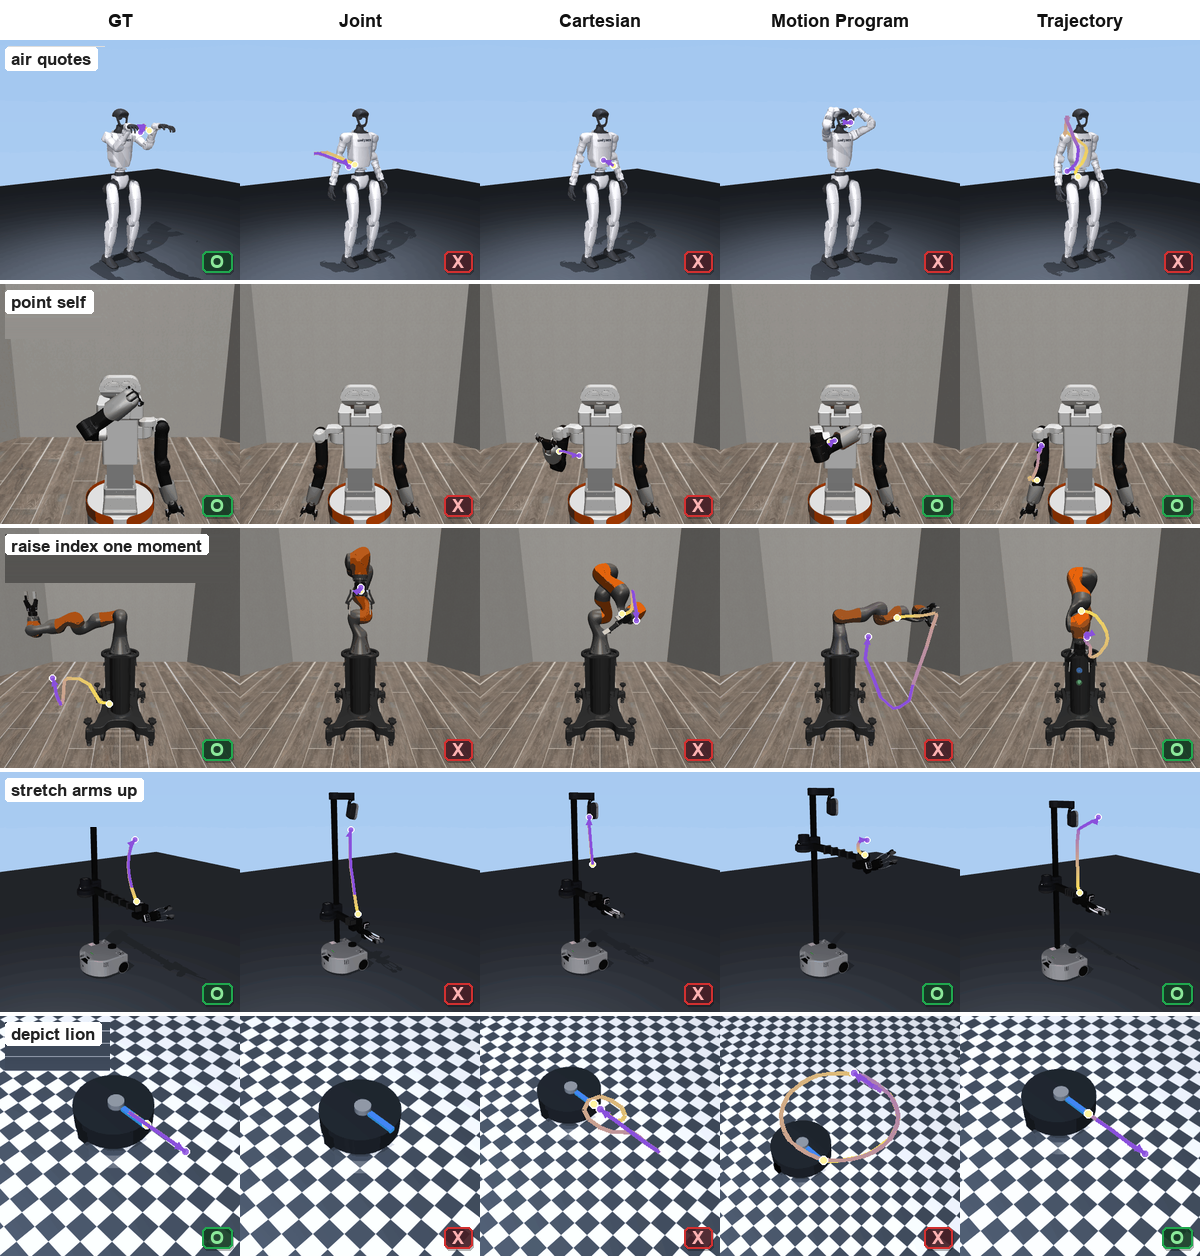
\includegraphics[width=.98\columnwidth]{figures/figure5_cross_embodiment_qualitative.png}
\caption{No single interface preserves the cue-bearing factors on every embodiment. Rows show Humanoid air quotes, Tiago point self, IIWA raise index one moment, Stretch stretch arms up, and Roomba depict lion; columns compare human-authored GT, \jointseq{}, \cartseq{}, \method{}, and \traj{}. Paths mark the active EE or base handle, and O/X denotes recognition.}
\label{fig:humanlike-qual}
\end{figure}

\subsection{Non-human-like Bodies}
Without a palm or a second hand these bodies must carry a cue through the path itself. Recognition is flatter than on the human-like bodies --- on Roomba the four interfaces span only 40.0--60.0\% (Fig.~\ref{fig:human}) --- and the cue profile inverts: deictic cues become the \emph{best} family on Roomba (60.7\%) while head and face cues become the worst (53.6\%; Table~\ref{tab:categories}).
\begin{itemize}
\item \textbf{Placement is comparable; orientation is not.} Location errors on Single Arm sit in the same band as the human-like bodies (14.2--34.2 percentile points), and \method{} is again the most accurate on every axis (Table~\ref{tab:factor-fidelity}). Orientation is where the interfaces come apart: \traj{} misses the tool-forward axis by 104.7\textdegree{}, past a right angle, so the gripper points away from where the reference points --- the worst cell in the table --- and with no gaze or second hand nothing disambiguates it.
\item \textbf{What is missing is richness, and that is what makes the motion bland.} Human-authored motion uses more coordinate directions than any interface on these bodies (38\% vs.\ 30--32\%; Table~\ref{tab:diversity}). \traj{} activates \emph{more} channels than a person (80 vs.\ 71) yet still fewer directions: it moves a lot, in the same few directions. The result is motion that is never wrong and never distinctive --- underspecification rather than misspecification.
\item \textbf{Prompting does not supply the missing richness.} Naming a confusable foil leaves victory, surrender, high-five, and fist-pump on the same radial strokes and loops (Fig.~\ref{fig:roomba-contrastive}); it bends the curvature locally without adding the lead-in, return, pause, or repetition that separates one path cue from another. Path cues do transfer where the body affords them --- \texttt{draw\_circle\_repeat} is recognized more often on the non-human-like bodies than on the human-like ones (92\% vs.\ 62\%) --- whereas posture cues collapse (\texttt{cover\_yawn\_sleepy}, 8\% vs.\ 50\%; Fig.~\ref{fig:cue-difficulty}).
\end{itemize}


\begin{figure}[t]
\centering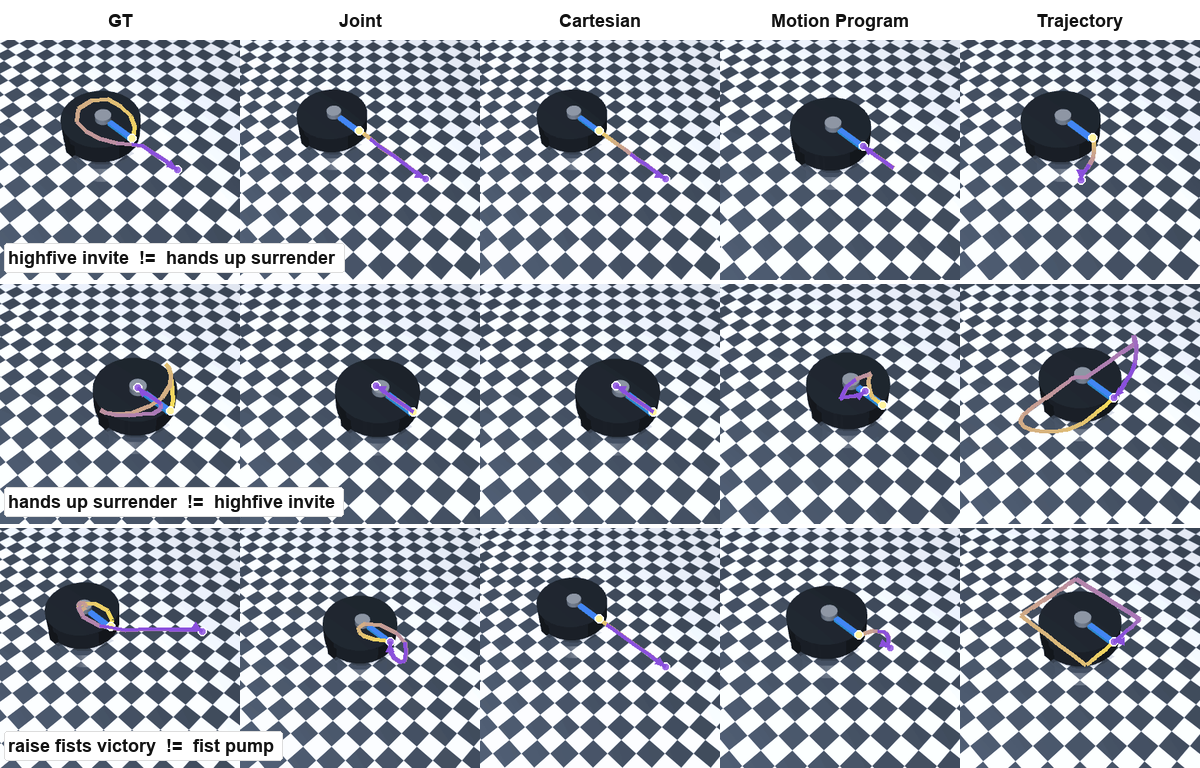
\includegraphics[width=.98\columnwidth]{figures/figure_roomba_contrastive.png}
\caption{Contrastive prompting does not reliably diversify Roomba paths. In the same five-column format as Fig.~\ref{fig:humanlike-qual}, each row requests a target cue distinguishable from a named foil; the overlays still reuse radial strokes and loops across semantic contrasts.}
\label{fig:roomba-contrastive}
\end{figure}

\begin{table}[t]
\caption{Expression diversity (\%): the share of landmarks (Chan.) and of coordinate directions (Dir.) that are active. Human-authored motion is the reference, and \textbf{bold marks the interface closest to it}, since neither more nor less motion is better in itself. Diversity is not conditioned on recognition. Human-like pools Humanoid and Tiago; Non-humanoid pools Stretch and Roomba.}
\label{tab:diversity}
\centering\footnotesize
\setlength{\tabcolsep}{3.5pt}
\renewcommand{\arraystretch}{1.1}
\begin{tabular}{l|cc|cc|cc}\toprule
& \multicolumn{2}{c|}{Human-like} & \multicolumn{2}{c|}{Single Arm} & \multicolumn{2}{c}{Non-humanoid}\\
Method & Chan. & Dir. & Chan. & Dir. & Chan. & Dir.\\\midrule
Cartesian-Space &32&28&80&72&\textbf{69}&30\\
Joint-Space &31&30&79&66&68&\textbf{32}\\
Motion Program &\textbf{22}&\textbf{14}&\textbf{63}&\textbf{46}&68&31\\
Trajectory Sketching &45&41&80&76&80&\textbf{32}\\\midrule
Human-authored &21&13&48&30&71&38\\\bottomrule
\end{tabular}
\end{table}

\section{Why Abstraction Matters}
\subsection{Token Efficiency}
An abstraction is useful when it changes the practical cost of communicating motion. Dense \jointseq{} and \cartseq{} outputs grow approximately linearly with state width and frame count, whereas \texttt{repeat}, \texttt{speed}, and \texttt{hold} reuse symbolic structure and a trajectory sketch emits only selected handles. Under a length-matched 24-frame protocol, \jointseq{} and \cartseq{} require 1,890.2 and 1,961.8 mean output tokens, versus 656.0 for \traj{} and 73.2 for \method{}. Humanoid dense outputs consume about 151 tokens per frame, so a 65,536-token output budget covers only about 434 frames---54 seconds at 8 Hz, 14 seconds at 30 Hz, or 7 seconds at 60 Hz---before prompt and reasoning tokens. The advantage is therefore not merely prose over numbers; it is compositional reuse instead of full sequence serialization (Fig.~\ref{fig:tokens}).

\begin{figure}[t]
\centering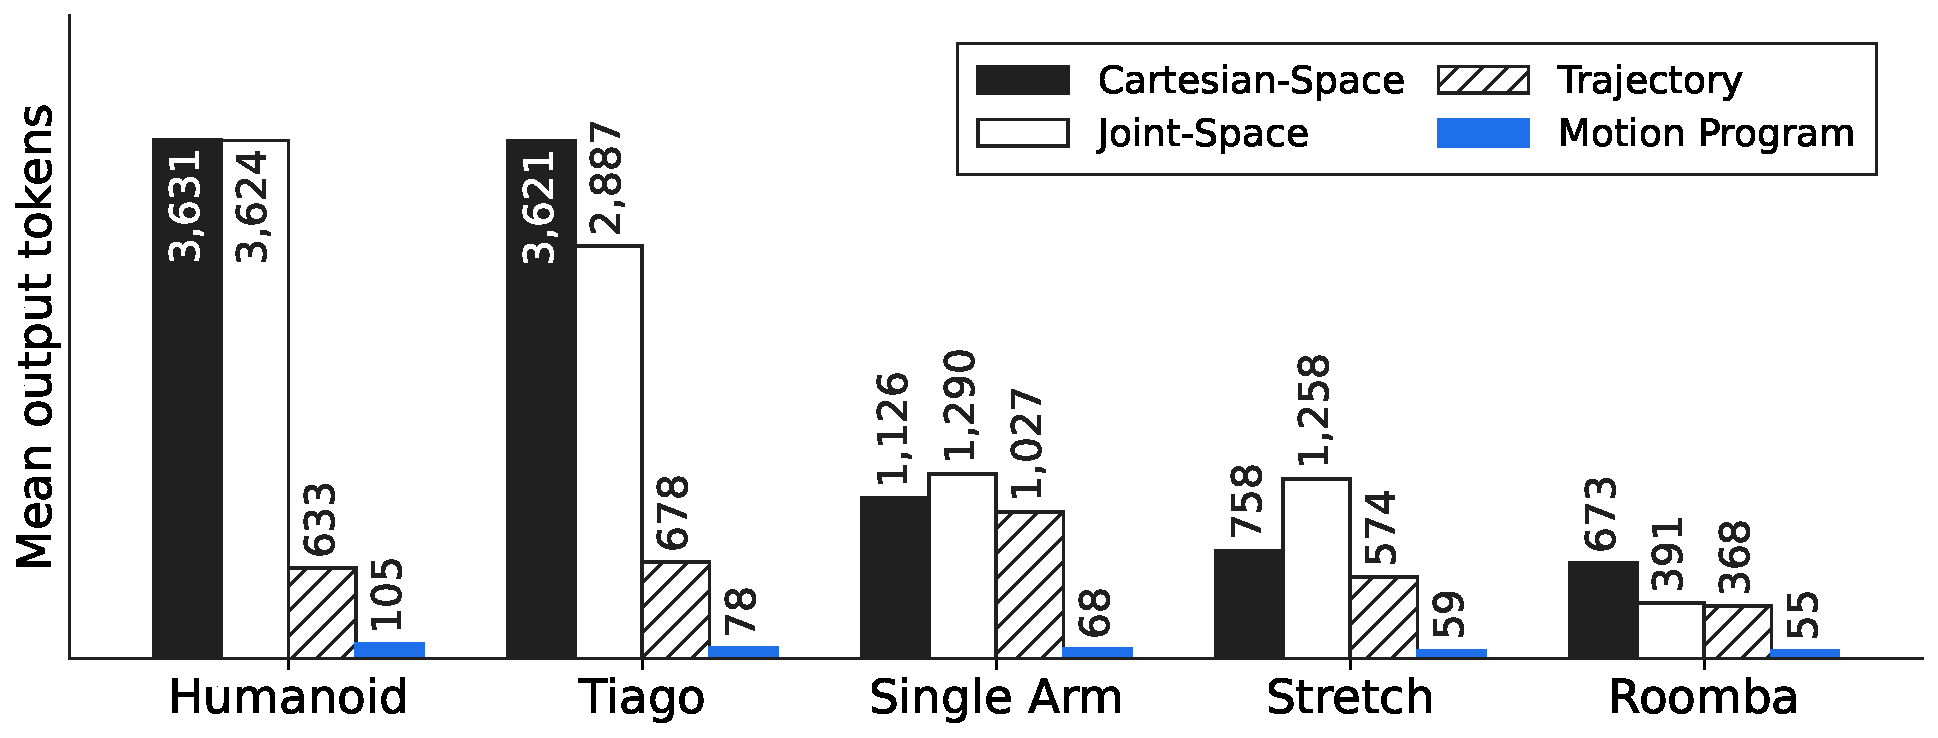
\includegraphics[width=.98\columnwidth]{figures/figure3_tokens.pdf}
\caption{Symbolic reuse sharply reduces output cost. Dense \jointseq{} and \cartseq{} serialization grows with trajectory width and duration, whereas \method{} fields compactly encode repetition, speed, and holds.}
\label{fig:tokens}
\end{figure}

\subsection{Inspectability and Communicability}
Abstraction also determines whether a person can inspect what the model intended and identify the factor that should be corrected. Dense state sequences expose only an executed result, while \method{} names editable pose/path factors and \traj{} exposes the selected geometric carrier. The qualitative differences make errors such as a wrong body-relative location, missing return, or insufficient path curvature directly discussable rather than hidden in a long numeric vector.

\section{Conclusion}
We introduced a controlled benchmark for a basic but under-isolated robotics question: how should language-model gesture knowledge be represented before execution on different bodies? Across five embodiments and four interfaces, dense numeric demonstrations are costly and brittle, while sparse symbolic and geometric interfaces preserve different semantic factors. The results argue for evaluating language-to-motion systems not only by trajectory similarity, but by the communicative factors and observer judgments that the representation preserves.

\begin{thebibliography}{99}
\bibitem{dragan2013legibility} A. D. Dragan, K. C. T. Lee, and S. S. Srinivasa, ``Legibility and predictability of robot motion,'' \emph{HRI}, 2013.
\bibitem{kopp2006bml} S. Kopp et al., ``Towards a common framework for multimodal generation: The Behavior Markup Language,'' \emph{IVA}, 2006.
\bibitem{salem2012gesture} M. Salem et al., ``Generation and evaluation of communicative robot gesture,'' \emph{International Journal of Social Robotics}, 2012.
\bibitem{chidambaram2012gesture} V. Chidambaram, Y.-H. Chiang, and B. Mutlu, ``Designing persuasive robots: How robots might persuade people using vocal and nonverbal cues,'' \emph{HRI}, 2012.
\bibitem{kucherenko2020gesticulator} T. Kucherenko et al., ``Gesticulator: A framework for semantically-aware speech-driven gesture generation,'' \emph{ICMI}, 2020.
\bibitem{yoon2020trimodal} Y. Yoon et al., ``Speech gesture generation from the trimodal context of text, audio, and speaker identity,'' \emph{ACM Trans. Graph. (SIGGRAPH Asia)}, 2020.
\bibitem{liu2022beat} X. Liu et al., ``BEAT: A large-scale semantic and emotional multi-modal dataset for conversational gestures,'' \emph{ECCV}, 2022.
\bibitem{ijspeert2013dmp} A. Ijspeert et al., ``Dynamical movement primitives,'' \emph{Neural Computation}, 2013.
\bibitem{paraschos2013promp} A. Paraschos et al., ``Probabilistic movement primitives,'' \emph{NeurIPS}, 2013.
\bibitem{calinon2016tpgmm} S. Calinon, ``A tutorial on task-parameterized movement learning and retrieval,'' \emph{Intelligent Service Robotics}, 2016.
\bibitem{stepputtis2020lcil} S. Stepputtis et al., ``Language-conditioned imitation learning for robot manipulation tasks,'' \emph{NeurIPS}, 2020.
\bibitem{brohan2023rt2} A. Brohan et al., ``RT-2: Vision-language-action models transfer web knowledge to robotic control,'' \emph{CoRL}, 2023.
\bibitem{liang2023cap} J. Liang et al., ``Code as policies: Language model programs for embodied control,'' \emph{ICRA}, 2023.
\bibitem{huang2023voxposer} W. Huang et al., ``VoxPoser: Composable 3D value maps for robotic manipulation,'' \emph{CoRL}, 2023.
\bibitem{dai2026lmp} Y. Dai et al., ``Language movement primitives: Grounding language models in robot motion,'' \emph{RSS}, 2026.
\bibitem{ling2026impact} J. Ling et al., ``IMPACT: Intelligent motion planning with acceptable contact trajectories via vision-language models,'' \emph{ICRA}, 2026.
\bibitem{broad2017corrections} A. Broad et al., ``Real-time natural language corrections for assistive robotic manipulators,'' \emph{IJRR}, 2017.
\bibitem{sharma2022correcting} M. Sharma et al., ``Correcting robot plans with natural language feedback,'' \emph{RSS}, 2022.
\bibitem{shi2024yell} L. Shi et al., ``Yell at your robot: Improving on-the-fly from language corrections,'' \emph{RSS}, 2024.
\end{thebibliography}

\section*{Supplementary Material}
This section provides the complete cue inventory and the embodiment-specific grounding of the two abstractions. It remains part of the eight-page ICRA 2027 submission.

\begin{table*}[t]
\caption{Complete 30-cue benchmark, grouped by primary communicative family.}
\label{tab:all-cues}
\centering\footnotesize
\begin{tabular}{lp{.76\textwidth}}\toprule
Family & Cues\\\midrule
Head / face & \texttt{nod\_yes}, \texttt{shake\_head\_no}, \texttt{gaze\_shift\_avoid}, \texttt{tilt\_head\_curious}, \texttt{cover\_yawn\_sleepy}, \texttt{rub\_eye\_tired}, \texttt{facepalm}\\
Deictic / directed & \texttt{point\_you}, \texttt{point\_self}, \texttt{beckon\_come\_here}, \texttt{stop\_palm\_out}, \texttt{salute}, \texttt{raise\_index\_one\_moment}, \texttt{highfive\_invite}\\
Emblematic pose / action & \texttt{fist\_pump}, \texttt{shrug\_idk}, \texttt{flex\_bicep}, \texttt{air\_quotes}, \texttt{arms\_open\_welcome}, \texttt{hands\_up\_surrender}, \texttt{stretch\_arms\_up}, \texttt{raise\_fists\_victory}, \texttt{cross\_arms\_defensive}, \texttt{palms\_together\_thank\_you}, \texttt{draw\_circle\_repeat}\\
Depictive / iconic & \texttt{depict\_tree}, \texttt{depict\_big\_bowl}, \texttt{depict\_lion}, \texttt{depict\_small\_object}, \texttt{depict\_flying\_bird}\\\bottomrule
\end{tabular}
\end{table*}

\begin{table*}[t]
\caption{Embodiment-specific grounding of the two abstractions. DoF counts are the gesture DoF exposed to generation. The symbolic interface preserves the same factor types while changing their physical interpretation; the sketch retains only cue-bearing geometric carriers.}
\label{tab:grounding}
\centering\scriptsize
\setlength{\tabcolsep}{3pt}
\begin{tabular}{p{.08\textwidth}p{.16\textwidth}p{.16\textwidth}p{.27\textwidth}p{.24\textwidth}}\toprule
Embodiment & DoF & Available carriers & \method{} grounding & \traj{} focus\\\midrule
Humanoid & 19: torso 3, head 2, two 7-joint arms 14 & Head, torso, two arms, palm axes & Body-relative hand location; EE/palm facing; bilateral pose; hand-path axis, extent, speed, repetition & Active wrist/hand paths; remaining upper-body joints retargeted from the selected handles\\
Tiago & 18: base 3, torso lift 1, head 2, two 6-joint arms 12 & Head, torso lift, two arms, grippers, mobile base & Robot-relative face/shoulder/sternum anchors; gripper approach axis; arm or base path & Active gripper and, when cue-bearing, base waypoints\\
Single Arm & 7: one serial chain & One serial arm and gripper frame & EE location and tool-frame direction; single-arm path and timing & One EE position/direction trace\\
Stretch & 11: base 3, lift, extension, wrist 3, gripper, camera 2 & Base, lift, extension, wrist, gripper, camera & Height, reach, wrist attitude, base heading; path extent, reversal, speed, hold & Wrist/EE trace plus base staging when active\\
Roomba & 3: planar $(x,y)$ and yaw & Planar translation and yaw & No arm pose; path topology, signed turn, extent, speed, repetition, pause & Planar base waypoints and yaw\\\bottomrule
\end{tabular}
\end{table*}

\end{document}
